

\pgfplotsset{width=5cm,compat=1.18}

\tikzset{every picture/.style={line width=0.75pt}} %set default line width to 0.75pt        

\begin{tikzpicture}[x=0.75pt,y=0.75pt,yscale=-1,xscale=1]
%uncomment if require: \path (0,300); %set diagram left start at 0, and has height of 300

%Image [id:dp0011035212048724485] 
\draw (307.8,139.93) node  {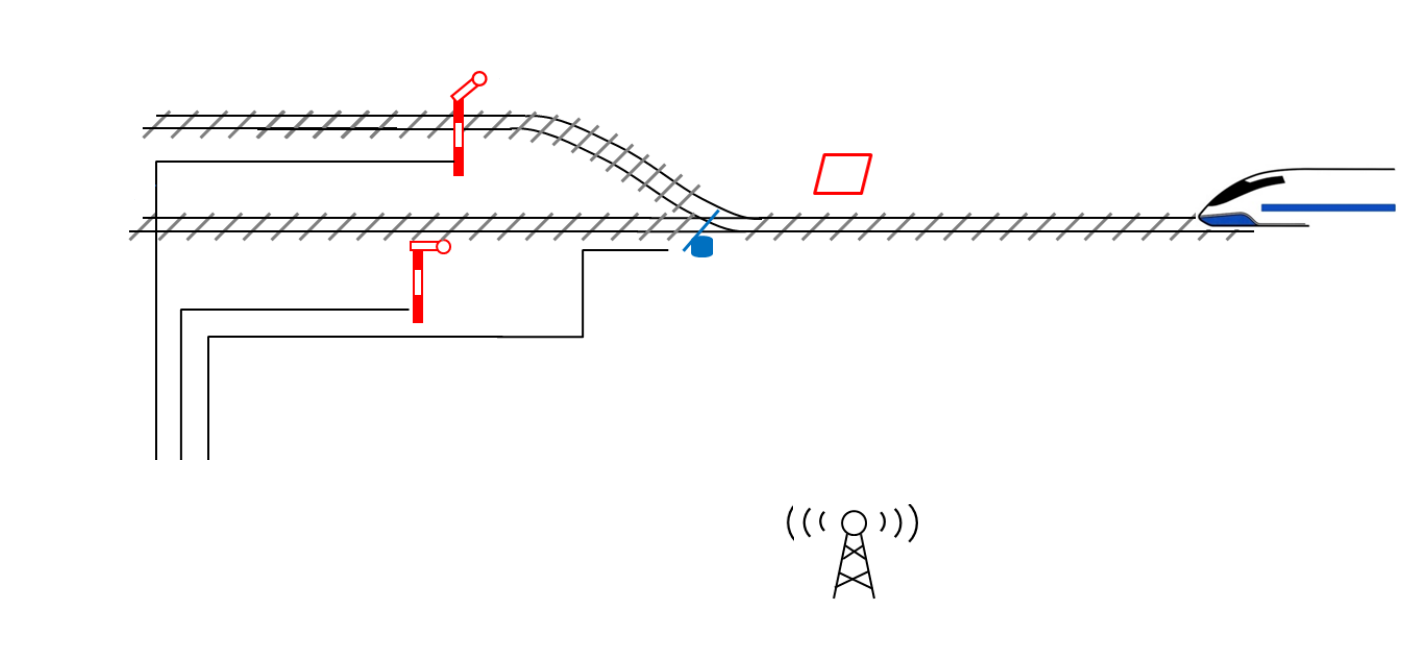
\includegraphics[width=350.8pt,height=176.4pt]{Part3/figure/railwayNetwork.png}};
%Rounded Rect [id:dp8635061097341326] 
\draw   (104.33,199.93) .. controls (104.33,192.79) and (110.12,187) .. (117.27,187) -- (156.07,187) .. controls (163.21,187) and (169,192.79) .. (169,199.93) -- (169,245.4) .. controls (169,252.54) and (163.21,258.33) .. (156.07,258.33) -- (117.27,258.33) .. controls (110.12,258.33) and (104.33,252.54) .. (104.33,245.4) -- cycle ;
%Right Arrow [id:dp5902707358380477] 
\draw   (169,199.93) -- (225.4,199.93) -- (225.4,191.7) -- (263,208.17) -- (225.4,224.63) -- (225.4,216.4) -- (169,216.4) -- cycle ;
%Rounded Rect [id:dp6848372643216789] 
\draw   (261.67,195.93) .. controls (261.67,188.79) and (267.46,183) .. (274.6,183) -- (313.4,183) .. controls (320.54,183) and (326.33,188.79) .. (326.33,195.93) -- (326.33,241.4) .. controls (326.33,248.54) and (320.54,254.33) .. (313.4,254.33) -- (274.6,254.33) .. controls (267.46,254.33) and (261.67,248.54) .. (261.67,241.4) -- cycle ;
%Right Arrow [id:dp00995349944529833] 
\draw   (261.74,249.63) -- (205.34,250.14) -- (205.42,258.37) -- (167.67,242.24) -- (205.12,225.44) -- (205.2,233.67) -- (261.59,233.17) -- cycle ;
%Right Arrow [id:dp13455094966677605] 
\draw   (369.29,188.62) -- (418.51,139.44) -- (412.87,133.8) -- (456.96,112.29) -- (435.42,156.36) -- (429.78,150.72) -- (380.57,199.9) -- cycle ;
%Right Arrow [id:dp26740738968744493] 
\draw   (488.46,128.23) -- (428.65,190.74) -- (434.41,196.25) -- (383.01,226.89) -- (411.36,174.2) -- (417.12,179.71) -- (476.94,117.21) -- cycle ;

% Text Node
\draw    (238.6,28.4) -- (277.6,28.4) -- (277.6,49.4) -- (238.6,49.4) -- cycle  ;
\draw (239.6,29.4) node [anchor=north west][inner sep=0.75pt]  [font=\footnotesize] [align=left] {signal};
% Text Node
\draw    (364.6,37.73) -- (404.6,37.73) -- (404.6,75.73) -- (364.6,75.73) -- cycle  ;
\draw (365.6,38.73) node [anchor=north west][inner sep=0.75pt]  [font=\footnotesize] [align=left] {virtual\\signal};
% Text Node
\draw    (311.93,111.07) -- (352.93,111.07) -- (352.93,132.07) -- (311.93,132.07) -- cycle  ;
\draw (312.93,112.07) node [anchor=north west][inner sep=0.75pt]  [font=\footnotesize] [align=left] {switch};
% Text Node
\draw    (123.27,32.4) -- (192.27,32.4) -- (192.27,53.4) -- (123.27,53.4) -- cycle  ;
\draw (124.27,33.4) node [anchor=north west][inner sep=0.75pt]  [font=\footnotesize] [align=left] {track circuit};
% Text Node
\draw    (149.27,147.73) -- (192.27,147.73) -- (192.27,168.73) -- (149.27,168.73) -- cycle  ;
\draw (150.27,148.73) node [anchor=north west][inner sep=0.75pt]  [font=\footnotesize] [align=left] {cables};
% Text Node
\draw (115.33,211.33) node [anchor=north west][inner sep=0.75pt]   [align=left] {IS};
% Text Node
\draw (274.67,209.33) node [anchor=north west][inner sep=0.75pt]   [align=left] {RBC};
% Text Node
\draw (169,199.93) node [anchor=north west][inner sep=0.75pt]  [font=\footnotesize] [align=left] {element states};
% Text Node
\draw (190.67,232) node [anchor=north west][inner sep=0.75pt]  [font=\footnotesize] [align=left] {train data};
% Text Node
\draw (365.02,188.71) node [anchor=north west][inner sep=0.75pt]  [font=\footnotesize,rotate=-315.58] [align=left] {movement authority\\};
% Text Node
\draw (387.02,206.04) node [anchor=north west][inner sep=0.75pt]  [font=\footnotesize,rotate=-315.58] [align=left] {position, track requests\\};


\end{tikzpicture}


